% Generated by plsimcount.pfseeds -- do not edit; regenerate instead.
% figure: B-all-by-formula -- Every formula at measured r; median over seeds [1, 2, 3, 4, 5], bars = min..max
% metric=t gatebase=ct merged
% seed 1: git_commit=8dd1b68c1faeffb1fb64439f6d7c9c5df3cf51a5 git_dirty=False
% seed 2: git_commit=8dd1b68c1faeffb1fb64439f6d7c9c5df3cf51a5 git_dirty=False
% seed 3: git_commit=8dd1b68c1faeffb1fb64439f6d7c9c5df3cf51a5 git_dirty=False
% seed 4: git_commit=8dd1b68c1faeffb1fb64439f6d7c9c5df3cf51a5 git_dirty=False
% seed 5: git_commit=8dd1b68c1faeffb1fb64439f6d7c9c5df3cf51a5 git_dirty=False
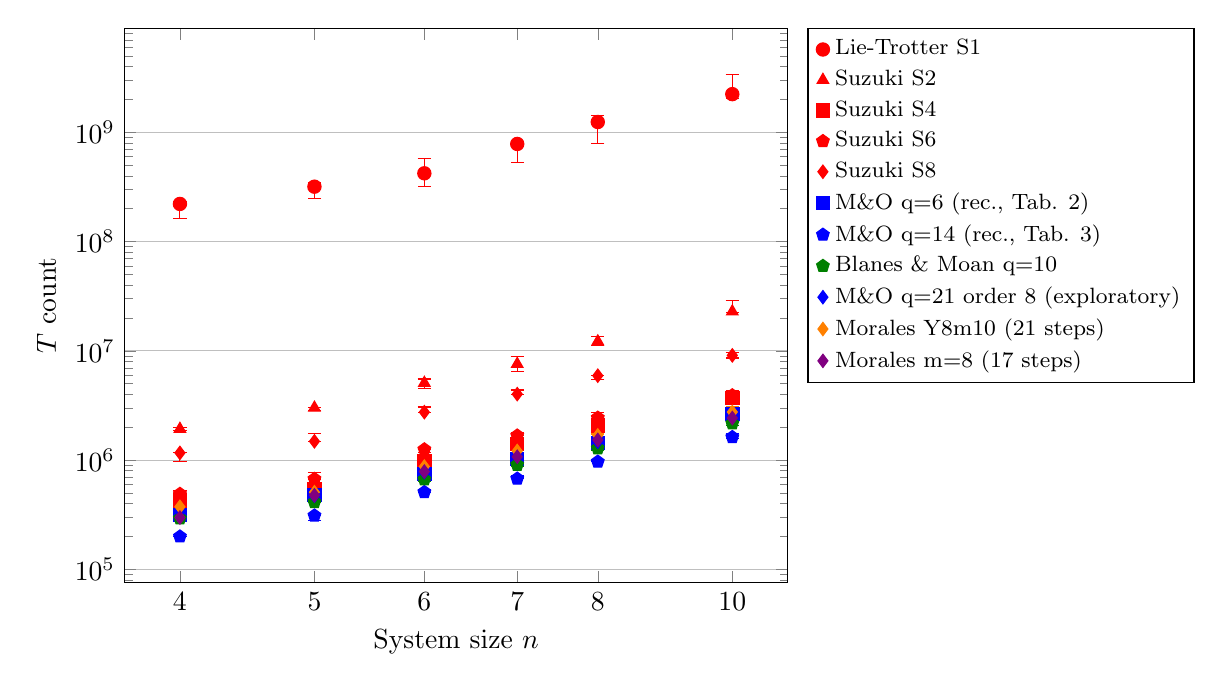
\begin{tikzpicture}
  \begin{loglogaxis}[
    width=10cm,
    xlabel={System size $n$},
    ylabel={$T$ count},
    xtick={4,5,6,7,8,10},
    xticklabels={4,5,6,7,8,10},
    ymajorgrids=true,
    legend pos=outer north east,
    legend cell align=left,
    legend style={font=\footnotesize},
  ]
    \addplot[only marks, red, mark=*, mark size=2.4pt, mark options={solid, fill=red}, error bars/.cd, y dir=both, y explicit, error bar style={red}] coordinates {
      (4,221263504) += (0,9069896) -= (0,57191984)
      (5,318348120) += (0,25613720) -= (0,71149566)
      (6,422071546) += (0,150465926) -= (0,104463980)
      (7,783651672) += (0,13465684) -= (0,255736656)
      (8,1244572288) += (0,196329224) -= (0,447938996)
      (10,2238616720) += (0,1152727882) -= (0,211682584)
    };
    \addlegendentry{Lie-Trotter S1}
    \addplot[only marks, red, mark=triangle*, mark size=2.4pt, mark options={solid, fill=red}, error bars/.cd, y dir=both, y explicit, error bar style={red}] coordinates {
      (4,1927848) += (0,51480) -= (0,62594)
      (5,3015896) += (0,41928) -= (0,159878)
      (6,5084160) += (0,449116) -= (0,552112)
      (7,7580986) += (0,1287530) -= (0,1106698)
      (8,12184250) += (0,1241932) -= (0,912938)
      (10,22892562) += (0,6036462) -= (0,613252)
    };
    \addlegendentry{Suzuki S2}
    \addplot[only marks, red, mark=square*, mark size=2.4pt, mark options={solid, fill=red}, error bars/.cd, y dir=both, y explicit, error bar style={red}] coordinates {
      (4,413718) += (0,5272) -= (0,742)
      (5,547344) += (0,73710) -= (0,24870)
      (6,983882) += (0,33568) -= (0,66258)
      (7,1405320) += (0,220920) -= (0,90456)
      (8,2071296) += (0,126240) -= (0,50016)
      (10,3700064) += (0,450366) -= (0,118640)
    };
    \addlegendentry{Suzuki S4}
    \addplot[only marks, red, mark=pentagon*, mark size=2.4pt, mark options={solid, fill=red}, error bars/.cd, y dir=both, y explicit, error bar style={red}] coordinates {
      (4,490724) += (0,40968) -= (0,520)
      (5,672420) += (0,98108) -= (0,896)
      (6,1253994) += (0,1680) -= (0,79154)
      (7,1677264) += (0,122664) -= (0,4896)
      (8,2442300) += (0,271290) -= (0,100376)
      (10,3919472) += (0,396598) -= (0,115280)
    };
    \addlegendentry{Suzuki S6}
    \addplot[only marks, red, mark=diamond*, mark size=2.4pt, mark options={solid, fill=red}, error bars/.cd, y dir=both, y explicit, error bar style={red}] coordinates {
      (4,1164480) += (0,4188) -= (0,187970)
      (5,1485780) += (0,263786) -= (0,2340)
      (6,2749626) += (0,314354) -= (0,4482)
      (7,4021776) += (0,362808) -= (0,4268)
      (8,5928020) += (0,9996) -= (0,415968)
      (10,9094694) += (0,574114) -= (0,479014)
    };
    \addlegendentry{Suzuki S8}
    \addplot[only marks, blue, mark=square*, mark size=2.4pt, mark options={solid, fill=blue}, error bars/.cd, y dir=both, y explicit, error bar style={blue}] coordinates {
      (4,314160) += (0,140) -= (0,840)
      (5,478632) += (0,1512) -= (0,10248)
      (6,744332) += (0,23116) -= (0,23804)
      (7,1018944) += (0,66240) -= (0,75708)
      (8,1435896) += (0,99144) -= (0,93708)
      (10,2628360) += (0,81736) -= (0,101208)
    };
    \addlegendentry{M\&O q=6 (rec., Tab. 2)}
    \addplot[only marks, blue, mark=pentagon*, mark size=2.4pt, mark options={solid, fill=blue}, error bars/.cd, y dir=both, y explicit, error bar style={blue}] coordinates {
      (4,199760) += (0,160) -= (0,160)
      (5,310728) += (0,576) -= (0,30536)
      (6,509696) += (0,28660) -= (0,896)
      (7,676620) += (0,40250) -= (0,792)
      (8,966504) += (0,40712) -= (0,1056)
      (10,1623768) += (0,124880) -= (0,54200)
    };
    \addlegendentry{M\&O q=14 (rec., Tab. 3)}
    \addplot[only marks, green!50!black, mark=pentagon*, mark size=2.4pt, mark options={solid, fill=green!50!black}, error bars/.cd, y dir=both, y explicit, error bar style={green!50!black}] coordinates {
      (4,293040) += (0,400) -= (0,240)
      (5,412544) += (0,88) -= (0,176)
      (6,665144) += (0,812) -= (0,22488)
      (7,905124) += (0,18928) -= (0,29348)
      (8,1281920) += (0,13352) -= (0,46400)
      (10,2164520) += (0,83880) -= (0,83108)
    };
    \addlegendentry{Blanes \& Moan q=10}
    \addplot[only marks, blue, mark=diamond*, mark size=2.4pt, mark options={solid, fill=blue}, error bars/.cd, y dir=both, y explicit, error bar style={blue}] coordinates {
      (4,338800) += (0,396) -= (0,176)
      (5,472704) += (0,840) -= (0,41240)
      (6,776608) += (0,48844) -= (0,960)
      (7,1092082) += (0,66918) -= (0,1178)
      (8,1472372) += (0,131116) -= (0,2420)
      (10,2481066) += (0,243350) -= (0,3074)
    };
    \addlegendentry{M\&O q=21 order 8 (exploratory)}
    \addplot[only marks, orange, mark=diamond*, mark size=2.4pt, mark options={solid, fill=orange}, error bars/.cd, y dir=both, y explicit, error bar style={orange}] coordinates {
      (4,374016) += (0,30258) -= (0,168)
      (5,509080) += (0,45824) -= (0,78)
      (6,873468) += (0,52174) -= (0,48356)
      (7,1213044) += (0,123118) -= (0,60244)
      (8,1684300) += (0,50212) -= (0,79468)
      (10,2757824) += (0,345592) -= (0,93560)
    };
    \addlegendentry{Morales Y8m10 (21 steps)}
    \addplot[only marks, violet, mark=diamond*, mark size=2.4pt, mark options={solid, fill=violet}, error bars/.cd, y dir=both, y explicit, error bar style={violet}] coordinates {
      (4,298032) += (0,48) -= (0,624)
      (5,477120) += (0,30944) -= (0,570)
      (6,786560) += (0,42646) -= (0,280)
      (7,1073318) += (0,874) -= (0,55642)
      (8,1529080) += (0,1120) -= (0,59416)
      (10,2429140) += (0,77108) -= (0,69064)
    };
    \addlegendentry{Morales m=8 (17 steps)}
  \end{loglogaxis}
\end{tikzpicture}
